\clearpage
\section{Simulation}
\label{sec:simulation}

\subsection{Robot model and scene}
The earlier Gazebo and MoveIt fixed-point pick-and-place project provided the development base. It established the robot model, collision scene, grasp approach, carrying motion, release, and return. Keyframe teaching and replay supported motion development before the six-grid task was integrated.\src{simulation}

The original \file{experiment3_sim_complete_20260914} used six red/blue cubes. The final extension, \file{experiment3_sim_bridge_20260921}, replaces the red cube in G2 and blue cube in G4 with two orange bridges. The six grid coordinates, other four objects, red/blue detection rules, original red/blue slots, and 65 mm carrying-centre height remain unchanged. The final scene has two red cubes, two blue cubes, and two bridges.\src{simcomplete,simbridge}

Each bridge is one 50 g rigid body with a crossbeam and two legs, three physical collision boxes, and a through-opening. Its envelope is $40\times40\times40$ mm; the opening is 20 mm wide and 28 mm high. Centre of mass and inertia are calculated from the component volumes. MoveIt conservatively uses the outer box for collision checking.

\begin{figure}[H]\centering
\begin{subfigure}{0.48\textwidth}
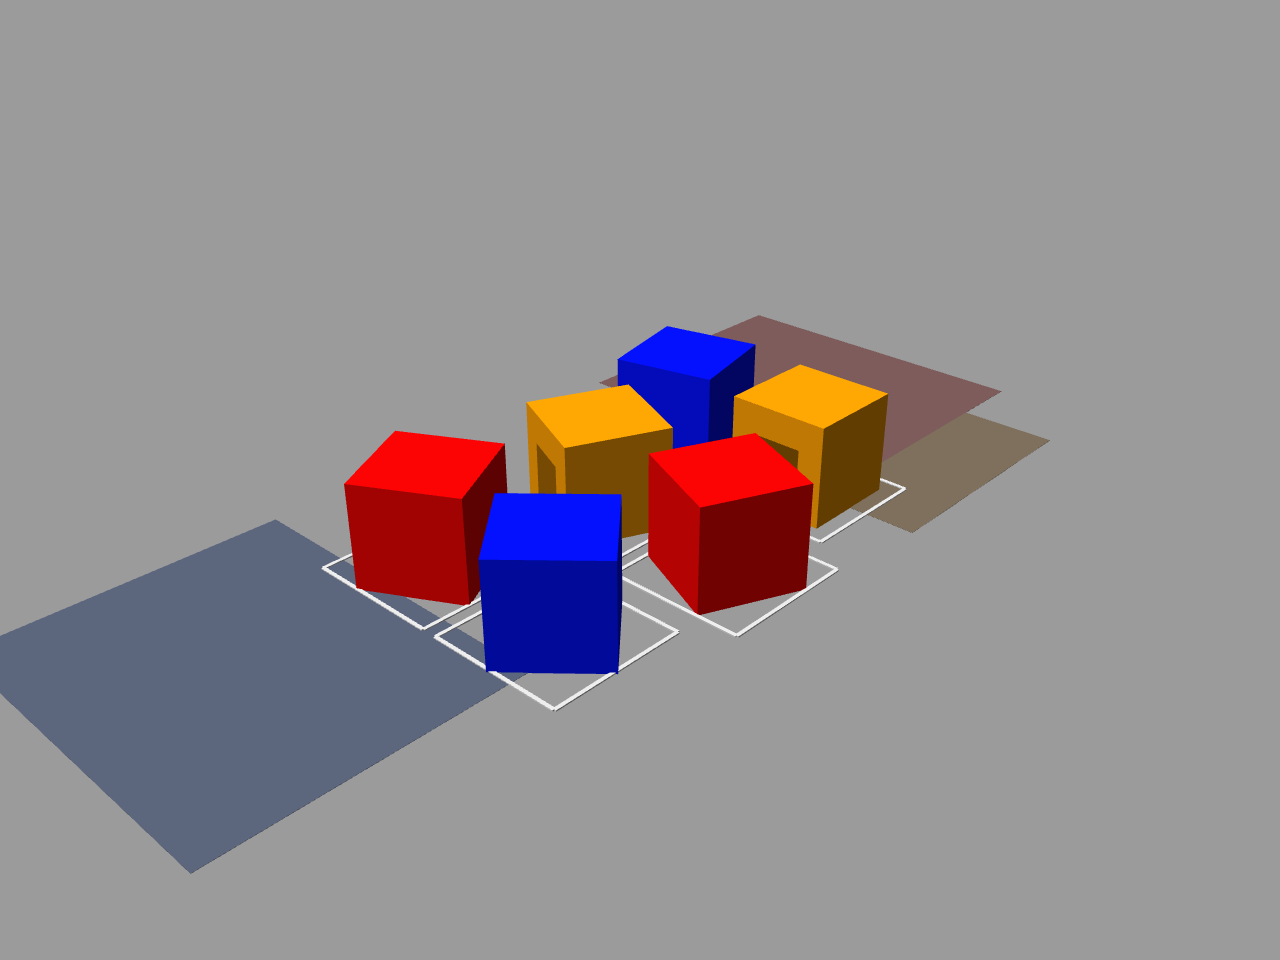
\includegraphics[width=\linewidth]{figures/simulation_bridge_initial.png}
\caption{Four cubes and two bridges in six source grids.}
\end{subfigure}\hfill
\begin{subfigure}{0.48\textwidth}
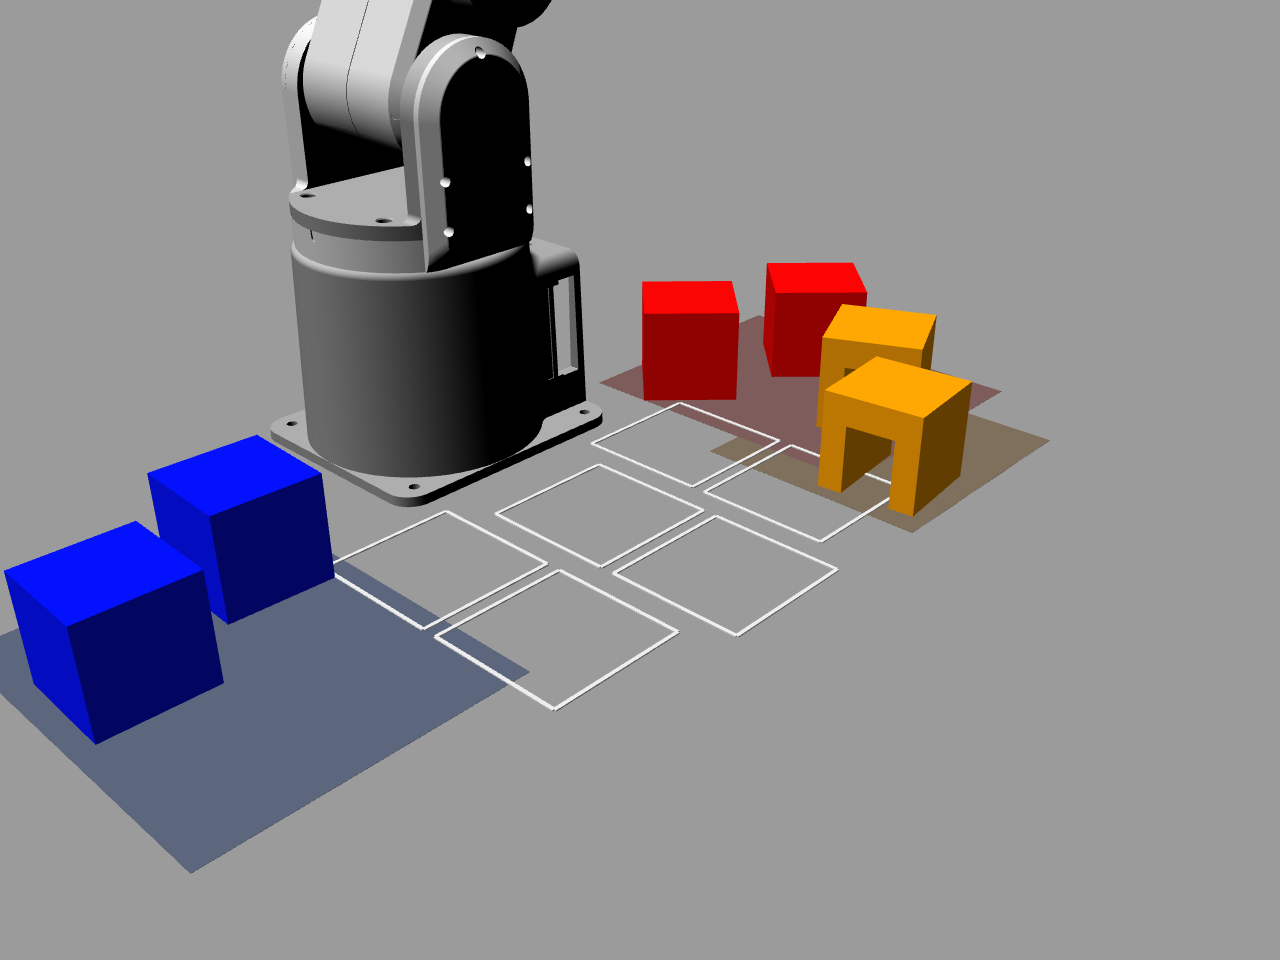
\includegraphics[width=\linewidth]{figures/simulation_bridge_final.png}
\caption{Final placement after six successful transfers.}
\end{subfigure}
\caption{Actual Gazebo side-camera images from the final bridge run. This observer camera does not participate in task decisions.}
\end{figure}

\subsection{Scene, image detection, and grid mapping}
The scene contains the mechArm, gripper, table, six fixed source cells, red/blue destination slots, added bridge slots on the left, and an overhead RGB sensor. The camera publishes a $960\times720$ image on \file{/task3/camera/overhead/image_raw}. The configured image rate is 8 Hz, not a measured processing rate.\src{simbridge}

The final simulation uses HSV segmentation and contour filtering for \file{red_cube}, \file{blue_cube}, and \file{orange_bridge}. It publishes class labels, boxes, and scores as \file{vision_msgs/Detection2DArray} on \file{/task3/detections}. Detection uses camera pixels, not scene ground-truth labels. Box centres are matched to projected grid regions and colors select destinations. This is color-associated classification, not color-independent shape recognition.\src{simbridge}

The simulation requires four consecutive matching grid observations and uses a configured minimum score of 0.65 before selecting a target. These settings belong to the HSV simulation pipeline. The physical system instead uses YOLO11 six-class detection, red/pink refinement, calibrated image polygons, and five-out-of-seven group voting. The two detectors and their scores are not interchangeable.

\subsection{Automatic control and motion feedback}
The simulation state machine contains \file{WAIT_READY}, \file{OBSERVE}, \file{SELECT}, \file{EXECUTING}, \file{VERIFY}, \file{RECOVER}, \file{DONE}, and \file{STOPPED}. The controller selects an eligible grid, submits one grasp job, waits for the result, allows the scene to settle, and then observes the remaining cells. The configured normal run processes each of the six grids once. It does not use the physical controller's refill policy.\src{simcomplete}

The grasp bridge exchanges request, status, result, and cancellation messages with job IDs. This is an equivalent feedback-based long-running task interface, rather than a standard ROS 2 Action server. Motion feedback and a 180 s controller job timeout prevent the controller from issuing another transfer while an earlier one is outstanding.

MoveIt plans the approach, grasp, lift, transfer, release, and return motions with collision objects. A simulation grasp check verifies alignment and gripper closure before attaching the object with a fixed constraint. This attachment supports carrying without snapping the object to a new pose; it is not a measurement of real friction or gripping force. Joint-state sampling and monitored physical contacts provide additional run checks.\src{simcomplete}

The complete system starts from one \file{full_sorting.launch.py}, including the scene, robot controllers, planning system, detector, grasp bridge, task controller, and independent acceptance monitor. The normal run does not require manual class, source-cell, or destination selection after startup.

\subsection{Final two-shape acceptance}
The final result is saved in \file{results/bridge_20260921_222016/acceptance.json}. Independent evaluation of actual Gazebo positions reports \file{PASS} and \file{DONE}: all six objects, including both bridges, are correctly placed. The evaluator checks the final position of each object.\src{simbridgerun}

\begin{table}[H]\tabstart
\caption{Object-level results of the final bridge simulation}
\begin{tabularx}{\textwidth}{@{}L{1.2cm}Y L{4cm}L{3cm}@{}}
\toprule Grid & Object & Target XY (m) & Independent result\\\midrule
G1 & Blue cube & $(0.170,0.070)$ & Correct\\
G2 & Orange bridge & $(-0.140,0.125)$ & Correct\\
G3 & Red cube & $(-0.170,0.070)$ & Correct\\
G4 & Orange bridge & $(-0.094,0.164)$ & Correct\\
G5 & Red cube & $(-0.112,0.045)$ & Correct\\
G6 & Blue cube & $(0.112,0.045)$ & Correct\\\bottomrule
\end{tabularx}\end{table}

The final run records 37,831 joint samples, zero joint-limit violations, zero monitored unsafe contact pairs, zero failed jobs, and a wall-clock duration of 391.53 s. The second bridge slot centre is just outside the source-grid edge, next to G4 after it has been emptied. Existing red/blue routing is preserved and remains different from the physical cube/other mapping.

Saved evidence includes configuration, world geometry, detections, job results, motion and safety logs, and two videos. The overhead video contains 1,354 frames encoded at 8 fps; the side video contains 651 frames at 5 fps. The videos use their configured encoding rates; the task duration comes from the run log.

\subsection{Historical normal and exception runs}
The normal record is \file{results/normal_front_arc_04/acceptance.json}. Independent evaluation of final object positions reports all six objects in their color-specific destinations: three red cubes and three blue cubes. The run finishes in \file{DONE}, with 37,412 joint samples, no recorded joint-limit violations, and zero contact pairs classified as unsafe by the monitor. Its recorded wall-clock duration is 466.26 s.\src{simruns}

\begin{table}[H]\tabstart
\caption{Recorded simulation results for the configured same-shape scene}
\begin{tabularx}{\textwidth}{@{}L{4.2cm}Y Y@{}}
\toprule Item & Normal run & Exception run\\\midrule
Run directory & \file{normal_front_arc_04} & \file{exceptions_front_arc_03}\\
Task state / evaluator status & \file{DONE} / \file{PASS} & \file{DONE} / \file{PASS}\\
Correct placements & 6 of 6 color-labeled cubes & 2 normal targets sorted; designated exception cells handled\\
Joint-state samples & 37,412 & 18,069\\
Recorded joint-limit violations & 0 & 0\\
Monitored unsafe contact pairs & 0 & 0\\
Wall-clock duration & 466.26 s & 238.73 s\\
\bottomrule
\end{tabularx}
\end{table}

The exception record is \file{results/exceptions_front_arc_03/acceptance.json}. Grid 2 contains an unknown-color object, grid 3 is empty, grid 5 has an injected unreachable-target condition, and grid 6 has an injected grasp failure. The controller skips the unknown and empty cells and handles the two motion failures through recovery. The remaining two ordinary targets are sorted. This run tests the designated exception branches; its two placements are not a normal-task sorting accuracy of two out of six.\src{simruns}

Both run directories preserve detections, task states, motion events, grasp-interface records, safety logs, initial/final images, and video. The independent evaluator checks actual final object positions rather than relying only on the controller's success count. 

\subsection{Debugging and remaining work}
The first bridge tests exposed an unreachable placement point and a Gazebo crash during release. We moved constraint operations to the physics-update thread and checked the distant slot with collision-free IK queries. Moving that slot inward allowed all six transfers to finish without lowering the carrying height.\src{simbridge}

After the accepted run, \file{move_group} logged a segmentation fault during SIGINT shutdown, while Gazebo exited normally. This shutdown issue remains to be resolved. The earlier exception tests cover the original scene; the bridge version has completed the normal run but has not repeated those exception tests.
